\section{Wireframe Reconstruciton}\label{sec:pcwireframe}
Using light variations to infer shape has been used extensively in the past~\cite{Kender86shapefrom,Daum1998,Kutulakos2000}. The 3\hyp D reconstruction consists of several steps. First the images have to be rectified; a process achieved through a process called camera calibration. 

\paragraph*{Contour Tracking} Adaptive thresholding is used in order to identify the areas with different illumination; see  Fig. \ref{fig:wire3} for the thresholded image where the cone of the video\hyp light meets the cave walls. Selecting the right value for thresholding the image required some domain knowledge, and currently was perform per video sequence, by a human. Current experiments consider adjusting the threshold based on keeping a balance between the amount of light and dark areas, but that work is outside the scope of this paper.

During the next step, edge detection marks the boundaries between light and dark areas; see Fig. \ref{fig:wire4} for the boundaries of Fig. \ref{fig:wire2}. The OpenCV Canny edge detector~\cite{canny1986computational} is used to identify the edges marking the lighter area boundaries. As can be seen, the edge map is very noisy and thus not suitable for estimating the walls of the cave. A filter is applied to the contour list, eliminating  short contours. More specifically, for every contour, its bounding box is calculated and then only the highest fifth percentile is kept. While this method can eliminate elongated contours, experiments with the actual underwater cave video footage proved to not affect the main boundaries. The filtered contours can be seen in Fig. \ref{fig:wire5}. Figure \ref{fig:wire6} superimposes the filtered contours on the rectified image; the areas where the cone of light meets the cave walls are clearly identifiable. In addition, the area with acceptable lighting is  extracted for use at the motion estimation. The edge map of the boundaries is used then as input to a stereo reconstruction algorithm.

 \begin{figure}[h]
 	\centering
 	\fbox{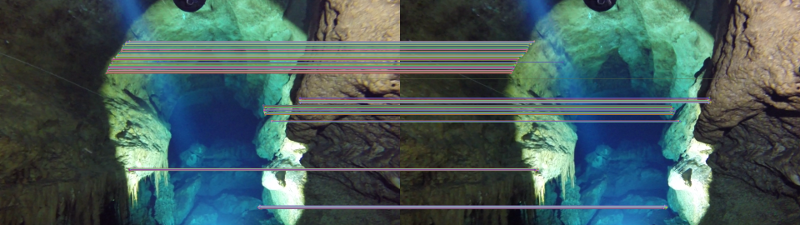
\includegraphics[width=.95\textwidth]{./figures/LT_0000_pngmatchesS}}
 	\caption{Select features matched at the boundary between left and right image of a stereo pair.}\vspace{-0.2in}
 	\label{fig:Matches}
 \end{figure}

\paragraph*{Sparse Stereo Reconstruction} The 3\hyp D structure of the cave boundaries is estimated for each stereo pair. For every point on the contour of the left image a SURF feature descriptor~\cite{Surf} is calculated using the left rectified image. Consequently, the same descriptor is matched on the right rectified image. Outlier rejection is facilitated by searching only locations at the same row and to the right of the left\hyp image feature's coordinates. As the camera calibration error is 0.8 pixels, it justifies the assumption above. Previous work on feature quality~\cite{ShiTomasi,Shkurti2011,RekleitisOceans2016} for underwater images indicated SURF~\cite{Surf} to be the most appropriate feature descriptor. Furthermore, the OpenCV Canny edge detector groups the edges in a list of continuous contours, as such consecutive points belonging to the same contour can be filtered for consistency.  Figure \ref{fig:Matches} presents select feature matches corresponding to the contours between the left and right image of a stereo pair.

\begin{figure*}[ht]
	\begin{center}
		\leavevmode
		\hspace*{-.2cm}\begin{tabular}{ccc}
			\subfloat[]{\fbox{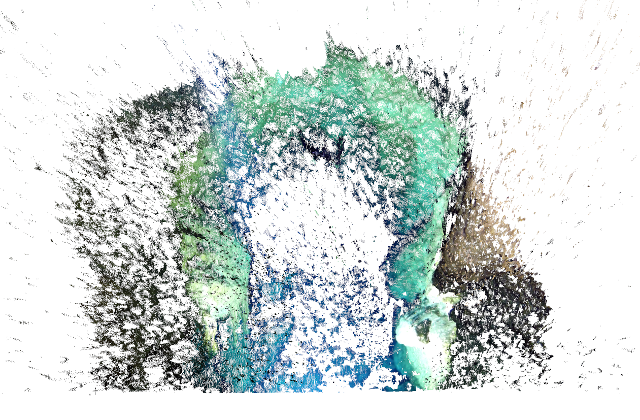
\includegraphics[height=0.14\textheight]{figures/sbm_straightS}}\label{fig:stereo1}}&
			\subfloat[]{\fbox{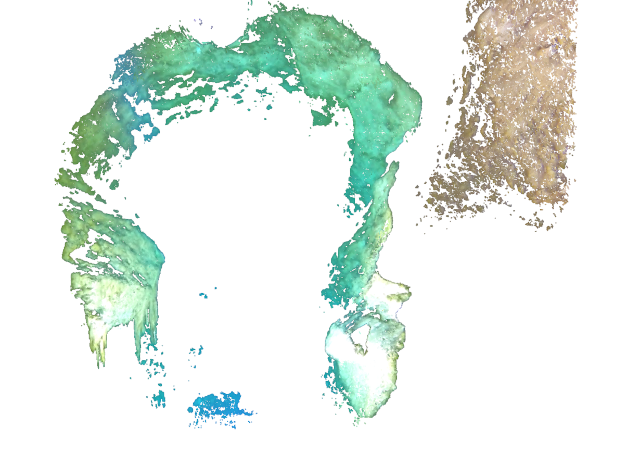
\includegraphics[height=0.14\textheight]{figures/threshold_straightS}}\label{fig:stereo2}}&
			\subfloat[]{\fbox{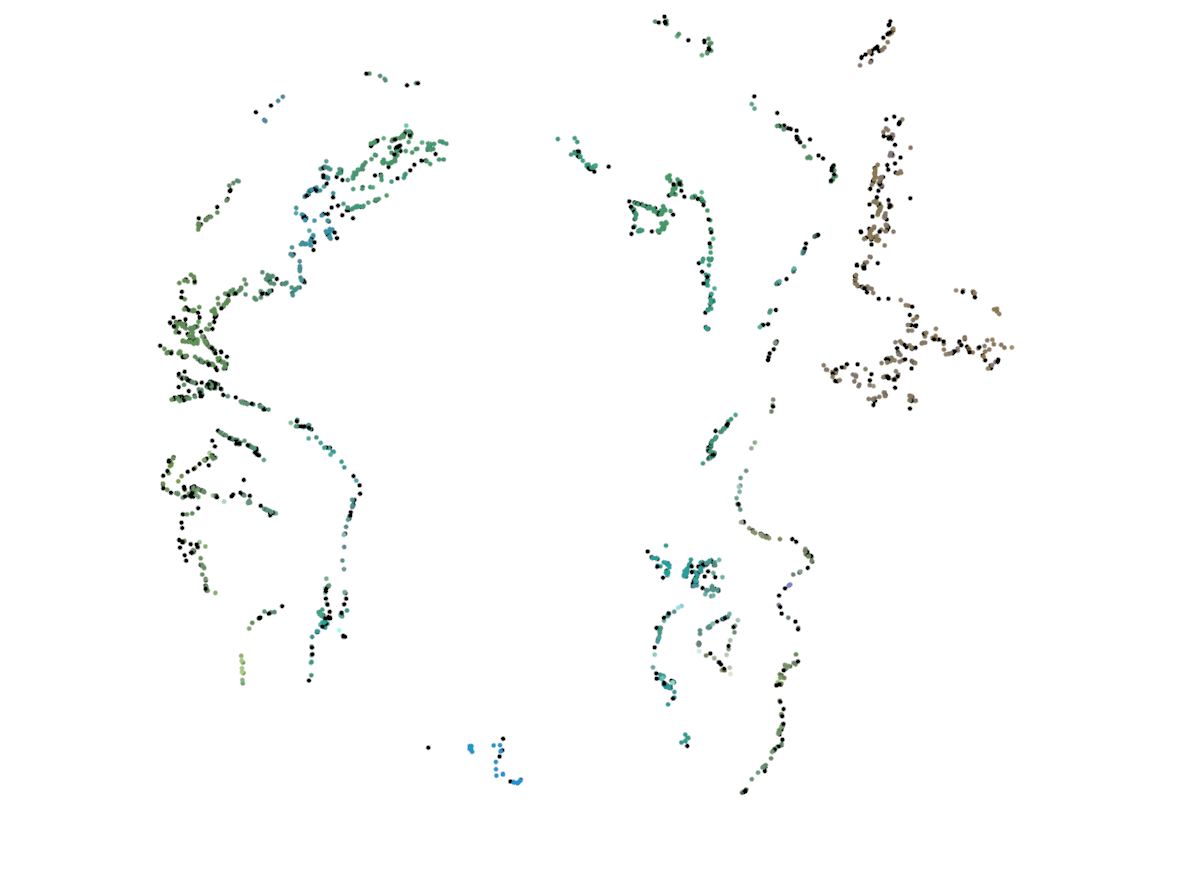
\includegraphics[height=0.14\textheight]{figures/contours_straight_larger}}\label{fig:stereo3}}\\
			\subfloat[]{\fbox{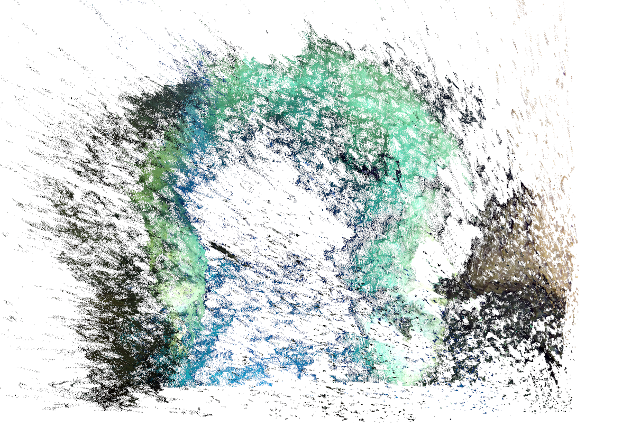
\includegraphics[height=0.14\textheight]{figures/sbm_shotgunS}}\label{fig:stereo4}}&
			\subfloat[]{\fbox{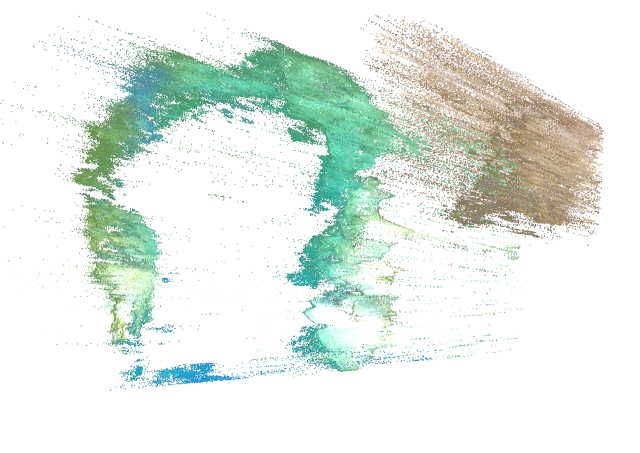
\includegraphics[height=0.14\textheight]{figures/threshold_shotgunS}}\label{fig:stereo5}}&
			\subfloat[]{\fbox{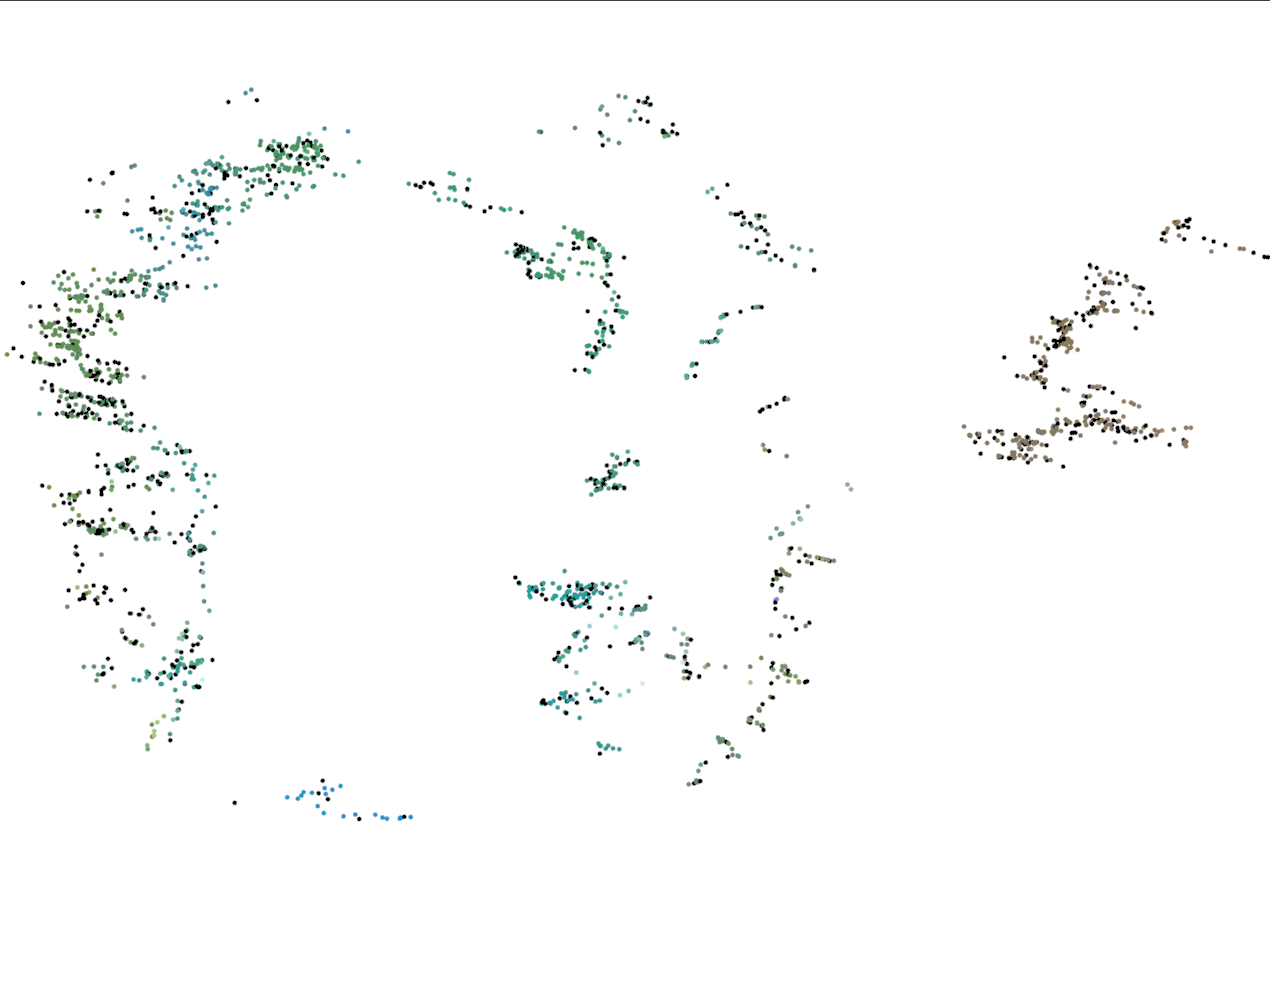
\includegraphics[height=0.14\textheight]{figures/contours_shotgun_larger}}\label{fig:stereo6}}
		\end{tabular}
	\end{center}
	\caption{Three different reconstructions from two different angles are presented. (a-c) Present a frontal view; (d-f) present a side view. \ref{fig:stereo1}, \ref{fig:stereo4} Disparity map of the Fig. \ref{fig:wire2} using the the OpenCV's semi-global block matching (SGBM) stereo algorithm.   \ref{fig:stereo2}, \ref{fig:stereo5} Applying the SGBM algorithm only to the lighted part.    \ref{fig:stereo3}, \ref{fig:stereo6} The contour in 3\hyp D using feature matches; see Fig. \ref{fig:Matches}. It is worth noting  elimination of outliers makes the contours much more distinct. }
	\label{fig:stereo}
\end{figure*}

Figure \ref{fig:stereo} presents a comparison of the performance of dense stereo reconstruction using OpenCV's semi-global block matching (SGBM) stereo algorithm~\cite{hirschmuller2008stereo} and the contour calculation. The standard output of dense stereo algorithms is a depth map, a normalized image where depth is quantified between 0 and 255; as such the values are discretized; see Figs. \ref{fig:stereo1},\ref{fig:stereo4} for the 3\hyp D reconstruction using the SGBM stereo algorithm on Fig. \ref{fig:wire2}. The noise is quite noticeable, Figs. \ref{fig:stereo2},\ref{fig:stereo5} present  the same reconstruction using only the lighted areas. Finally, Figs. \ref{fig:stereo3}, \ref{fig:stereo6} present  only the contours of high intensity variation extracted from Fig. \ref{fig:wire2} projected in 3\hyp D using SURF feature matching between left and right image. The noise is largely reduced, and the cave boundaries are clearly identifiable. While the first row of Fig. \ref{fig:stereo} presents a frontal view, and the error is not noticeable, the second row, presents a side view and the outliers are obvious. Currently, the corresponding points are calculated with pixel accuracy which results in disparity estimates that are integers. Consequently, the depth estimation is discretized and as it is inversely proportional to the distance of the camera there is a scattering effect. While this effect is strong during dense reconstructions, see Fig. \ref{fig:stereo3}, it is also present on the contour estimation; see Fig. \ref{fig:stereo4}